\section{Theoretischer Hintergrund}
\label{th}
In dieser Sektion werden wichtige Grundlagen definiert und anhand von Beispielen erläutert. Zunächst folgt eine Einführung in Artificial Neural Networks (zu Deutsch: \textit{Künstliche neuronale Netze}) in Sektion \ref{ann}. Daraufhin werden Convolutional Neural Networks (zu Deutsch etwa:\textit{Faltende neuronale Netze}) und ihre allgemeinen Bestandteile näher erklärt (Sektion \ref{cnn}). 

\subsection{Artificial Neural Networks}
\label{ann}
Artificial Neural Networks (ANNs) sind im Machine Learning (zu Deutsch: \textit{Maschinelles Lernen}) angewandte Techniken, die von biologischen neuronalen Netzen inspiriert sind.  

Machine Learning ist ein Bereich der Informatik, in dem man Probleme durch Algorithmen lösen möchte, welche keinen statisch programmierten Lösungsweg benötigen. Das Ziel von Machine Learning ist das Konstruieren von Algorithmen, die anhand von Datensätzen Schlussfolgerungen ziehen können und bei Eingabe unbekannter Daten diese Schlussfolgerungen zur Vorhersage von Ergebnissen generalisieren können.

ANNs können als gerichtete Graphen verstanden werden. Sie bestehen aus einer Menge an Knoten mit einer Menge an Kanten als Verbindungen zwischen den Knoten, welche die Aktivierungen der Knoten transportieren. Bei ANNs wird zwischen verschiedenen Strukturen unterschieden. In dieser Arbeit werden ausschließlich sogenannte Feed-Forward Neural Networks (zu deutsch etwa: \textit{vorwärts gekoppelte neuronale Netze}) genutzt. In Feed-Forward Neural Networks sind Knoten in Layern (zu Deutsch: \textit{Schichten}) angeordnet, welche untereinander kommunizieren. Ein Feed-Forward Neural Network ist immer ein gerichteter azyklischer Graph in dem die Signale der Neuronen in Kantenrichtung weitergegeben werden.

Neuronen in ANNs haben einen Bias und jede Verbindung zu anderen Neuronen ist mit einem Gewicht belegt. Die Werte beider Eigenschaften sind variabel und werden im Verlauf des Lernprozesses immer wieder angepasst. Außerdem verfügt jedes Neuron über eine Aktivierungsfunktion, welche die Ausgabe des Neurons abhängig vom Eingabewert definiert.

%Artificial neurons are assigned with a bias and connections between neurons have a weight assigned to them. Additionally, neurons have an activation function. An activation function defines the output of a node dependent on the given input. The output function is a function, that takes the computed activation and returns the final output, that is send to the next neuron. Artificial neurons are typically organized in layers. Those layers can perform different kinds of transformations of their inputs (e.g. pooling layers, convolutional layers, etc. when looking at CNNs). 



Abbildung \ref{fig:basictop} zeigt eine einfache Topologie eines ANNs. Eine Eingabe wird vom Input Layer (zu Deutsch: \textit{Eingabeschicht}) in den Hidden Layer (zu Deutsch: \textit{Versteckte Schicht}) gegeben und von diesem in die letzte Schicht, welche als Output Layer (zu Deutsch: \textit{Ausgabeschicht}) funktioniert weitergereicht. Der Hidden Layer kann aus mehreren unterschiedlichen Layern bestehen und dient lediglich als Abstraktion aller Schichten zwischen Input und Output Layer.

\begin{figure}[ht]
\centering
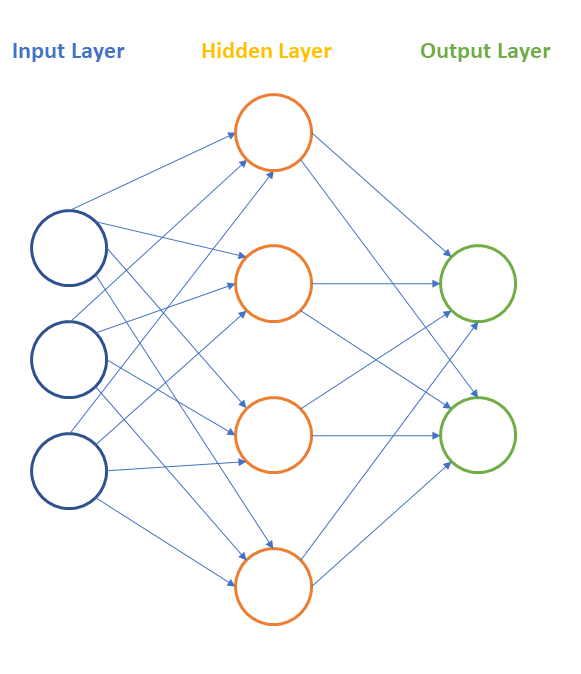
\includegraphics[scale=0.5]{pictures/grafiken/Folie3}
\caption[Caption for LOF]{Topologie eines einfachen ANNs.} 
\label{fig:basictop}
\end{figure}

Neural Networks (zu Deutsch: \textit{Neuronale Netze}) können als mathematische Modelle verstanden werden, welche eine Funktion $f : X \rightarrow Y$ definieren. In einem Neural Network wendet jedes Neuron eine Funktion auf seine Eingangswerte an, bevor es diese zur nächsten Schicht sendet. Somit kann die Funktion eines Neural Networks als eine Komposition aus jeder sich im Networks befindlichen Funktion definiert werden. 

Bezogen auf Abbildung \ref{fig:composedGraph}, sieht die zusammengesetzte Funktion des Networks wie folgt aus: 
\begin{equation}
\label{eq:compf}
f(g_1(h_1(x), h_2(x)),g_2(h_2(x), h_3(x)))
\end{equation}

\begin{figure}[ht]
\centering
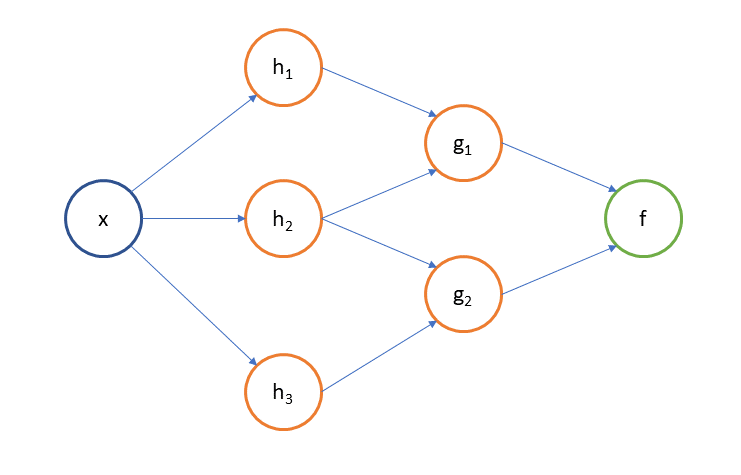
\includegraphics[scale=0.4]{pictures/grafiken/Folie4}
\caption[Caption for LOF]{Grafische Darstellung der zusammengesetzten Funktion $f$ aus Gleichung \ref{eq:compf}.}
\label{fig:composedGraph}

\end{figure}

\paragraph{Fully-Connected layer}
Jeder Layer in einem klassischen ANN ist ein Fully-Connected Layer (zu Deutsch etwa: \textit{vollständig verbundene Schicht}). Neuronen in Fully-Connected Layern besitzen Verbindungen zu allen Neuronen des vorrangigen Layers. Jedes Neuron berechnet einen Ausgabewert $F(x)$ unter Verwendung des Eingabewertes \vect{x}, der Gewichte \mat{W}, die den Verbindungen zu dem vorherigen Layer zugewiesen sind, und eines Bias \vect{b}, der dem entsprechenden Neuron zugewiesen ist. 
\begin{equation}
\label{eq:fcl}
\begin{bmatrix}
w_{11} & ... & w_{1m}\\
. &  & .\\
. & . & .\\
. &  & .\\
w_{n1} & ... & w_{nm} 
\end{bmatrix} \cdot
\begin{bmatrix}
x_1\\
.\\
.\\
.\\
x_m
\end{bmatrix} + 
\begin{bmatrix}
b_1\\
.\\
.\\
b_n
\end{bmatrix} = 
\begin{bmatrix}
y_1\\
.\\
.\\
y_n
\end{bmatrix}
\end{equation}
Gleichung \ref{eq:fcl} zeigt die allgemeine Formel nach welcher der Ausgabewert eines Fully-Connected Layers berechnet wird. $n$ steht für die Anzahl der Neuronen im Layer und $m$ ist die Anzahl der Eingabewerte des vorherigen Layers. Die Gleichung kann auch wie folgt in Vektornotation formuliert werden: 
\begin{equation}
\label{eq:VecNot}
F(\vect{x}) = (\mat{W} \cdot \vect{x}) + \vect{b}
\end{equation} 
In Gleichung \ref{eq:VecNot} sind \mat{W} und \vect{b} lernbare Parameter, welche vom Optimierungsalgorithmus abgepasst werden können. Sie stehen in der Gleichung für die Gewichte (\mat{W}) und den Bias (\vect{b}) des entsprechenden Layers.

\paragraph{Rectified Linear Units Layer}

In ANNs finden eine Vielzahl von Aktivierungsfunktionen Anwendung. Im Folgenden wir die ReLU-Funktion vorgestellt, da sie in den Modellen, die in dieser Arbeit implementiert werden genutzt wird. Sie ist wie folgt definiert: $relu(x) = max(0, x)$. Die Aktivierungsfunktion wird nach der Verarbeitung eingehender Werte im Neuron auf das Ergebnis angewandt und entfernt negative Werte aus dem Ausgabevektor des Neurons, bevor der Vektor an den nächsten Layer weitergereicht wird \parencite{Wu.2017}.

\paragraph{Normalization Layer}

Das Normalization Layer (zu Deutsch: \textit{Normalisierungsschicht}) wird zur Normalisierung der Aktivierungen des vorherigen Layers genutzt und dient unter anderem der Verhinderung von \textit{Overfitting} (zu Deutsch: Überanpassung). Overfitting tritt dann auf wenn ein Algorithmus die Trainingsdaten zu gut lernt und nicht mehr auf Grundlage dieser die Eingaben generalisieren kann. 

Nachfolgend wird ausschließlich Batch Normalization (BN) genutzt, da es sowohl für Fully-Connected Layer als auch für Convolutional Layer genutzt werden kann und die Trainingsgeschwindigkeit des Netzwerks beschleunigt \parencite{DBLP:conf/icml/IoffeS15}. Angewandt auf einen Mini-Batch $B$ mit den Eingaben $B = \{x_1...m\}$   berechnet Batch Normalization für eine n-dimensionale Eingabe $x = (x^{(1)} ... x^{(n)}) \in B$ zunächst den Mittelwert und die Varianz des Batches: 
\begin{equation}
	mean(B) = \frac{1}{m}\sum_{i=1}^{m} x_i
\end{equation}
\begin{equation}
	var^2(B) = \frac{1}{m}\sum_{i=1}^{m} (x_i - mean(B))^2 
\end{equation}

Mit beiden Werten wird die Eingabe dann Normalisiert, wobei $\epsilon$ als Konstante zur Varianz addiert wird um numerische Stabilität sicher zu stellen:

\begin{equation}
	\hat{x}_i = \frac{x_i - mean(B)}{\sqrt{var^2(B) + \epsilon}}
\end{equation}

Zuletzt wird die Eingabe skaliert und verschoben. $\gamma$ und $\beta$ sind lernbare Parameter, welche im Batch Normalization Layer eingeführt werden: 

\begin{equation}
	y_i = \gamma \times \hat{x}_i + \beta
\end{equation}


\paragraph{Loss Function}

Die Loss Function (zu Deutsch: \textit{Verlustfunktion}) evaluiert wie genau ein Neural Network die ground-truth (zu Deutsch etwa: Grundwahrheit) der Trainingsdaten vorhersagt. Ihre Aufgabe besteht darin den Abstand zwischen der ground-truth \vect{(x, y)} einer Eingabe \vect{x} und der Vorhersage des ANNs $\hat{y}$. Neural Networks versuchen Gewichte und Biase so anzupassen, dass dieser Wert minimiert wird. Ein Beispiel für eine Loss Function $z$ wäre \parencite{Wu.2017}:

\begin{equation}
z = \frac{1}{2}\|\vect{(x, y)} - \hat{\vect{y}}\|^2
\end{equation}


\paragraph{Softmax-Funktion}

Die Softmax-Funktion ist eine Variante der logisitschen Funktion. Die Funktion erh\"alt einen Vektor \vect{z} mit reellen Werten und einer beliebigen Dimension $K$ und verrechnet dessen Werte, so dass sich jeder Wert des Vektors \vect{z} im Bereich (0, 1] befindet und die Summe aller Werte 1 ergibt. Die Softmax-Funktion wird nach folgender Formel berechnet \parencite{Goodfellow-et-al-2016}:

\begin{equation}
softmax(\vect{z})_j = \frac{\mathrm{e}^{z_j}}{\sum_{k=1}^K \mathrm{e}^{z_k}}
\end{equation}

Eine vollständige Funktion für das in Abbildung \ref{fig:basictop} gezeigte ANN wird in Gleichung \ref{eq:annfunc} ausformuliert.
\begin{equation}
f(\mathbf{x}) = softmax(\mathbf{W_2} \cdot relu(\mathbf{W_1} \cdot \mathbf{x} + \mathbf{b_1}) + \mathbf{b_2} )
\label{eq:annfunc}
\end{equation}


Der Eingabevektor \vect{x} ist in $\mathbb{R}^3$. Zuerst wird \vect{x} vom Hidden Layer verarbeitet. In diesem Beispiel ist der Hidden Layer Fully-Connected, so dass die Formel für Fully-Connected Layer \ref{eq:fcl} mit $\mathbf{W_1}$ und $\mathbf{b_1}$ angewendet werden kann. $\mathbf{W_1}$ ist eine $4 \times 3$ Matrize und $\mathbf{b_1}$ ist in $\mathbb{R}^4$. Das Resultat wird mit einer Aktivierungsfunktion -- in diesem Fall der ReLU-Funktion -- verrechnet und hat danach die Dimension $4\times1$. Daraufhin wird das Resultat an den Output Layer weitergegeben, welcher auch ein Fully-Connected Layer ist. Auch hier wird Gleichung \ref{eq:fcl} für Fully-Connected mit $\mathbf{W_2}$ als $2\times4$ Matrix und $\mathbf{b_2}$ als Vektor in $\mathbb{R}^2$ angewandt. Zuletzt wird die Softmax-Funktion auf das Ergebnis des Output Layers angewandt. Die Dimension des Ausgabevektors ist $2\times1$.


\subsection{Convolutional Neural Networks}

\label{cnn}

Ein Convolutional Neural Network (CNN) ist eine Spezialisierung des allgemeineren ANN-Begriffs. Es findet häufig  Anwendung um Aufgaben im Zusammenhang mit Bildern, wie zum Beispiel Bildklassifikationen, zu lösen. Im Vergleich zu ANNs benötigen CNNs im Allgemeinen weniger Gewichte, durch ihre Eigenschaft der lokalen Konnektivität.

Ähnlich wie ANNs bestehen CNNs jeweils aus einem Input und einem Output Layer. Zwischen diesen beiden Layern befinden sich ein oder mehrere Hidden Layer, welche die Informationen aus den Eingabedaten verarbeiten. Die Hidden Layer können aus verschiedenen Layer-Typen zusammengesetzt werden, welche beliebig untereinander kombiniert werden können. Einige dieser Layer sind zum Beispiel: Convolutional, Pooling, Fully-Connected und Normalization Layer. In der Praxis sind ideale Layerzusammenstellungen stark an die Problemstellung gebunden und werden empirisch bestimmt. 

\paragraph{Tensor}

Ein Tensor wird im Kontext von Python und Tensorflow als ein mehrdimensionales Array verstanden. In der Arbeit werden drei- und vierdimensionale Tensoren verwendet. Abbildung \ref{fig:bth} zeigt eine visuelle Erklärung der Begriffe, die im Bezug auf Tensoren folgend genutzt werden. Breite beschreibt die Ausdehnung des Tensors auf der x-Achse, Höhe die Ausdehnung auf der y-Achse und die Tiefe die Ausdehnung auf der z-Achse. 

\begin{figure}[H]
\centering
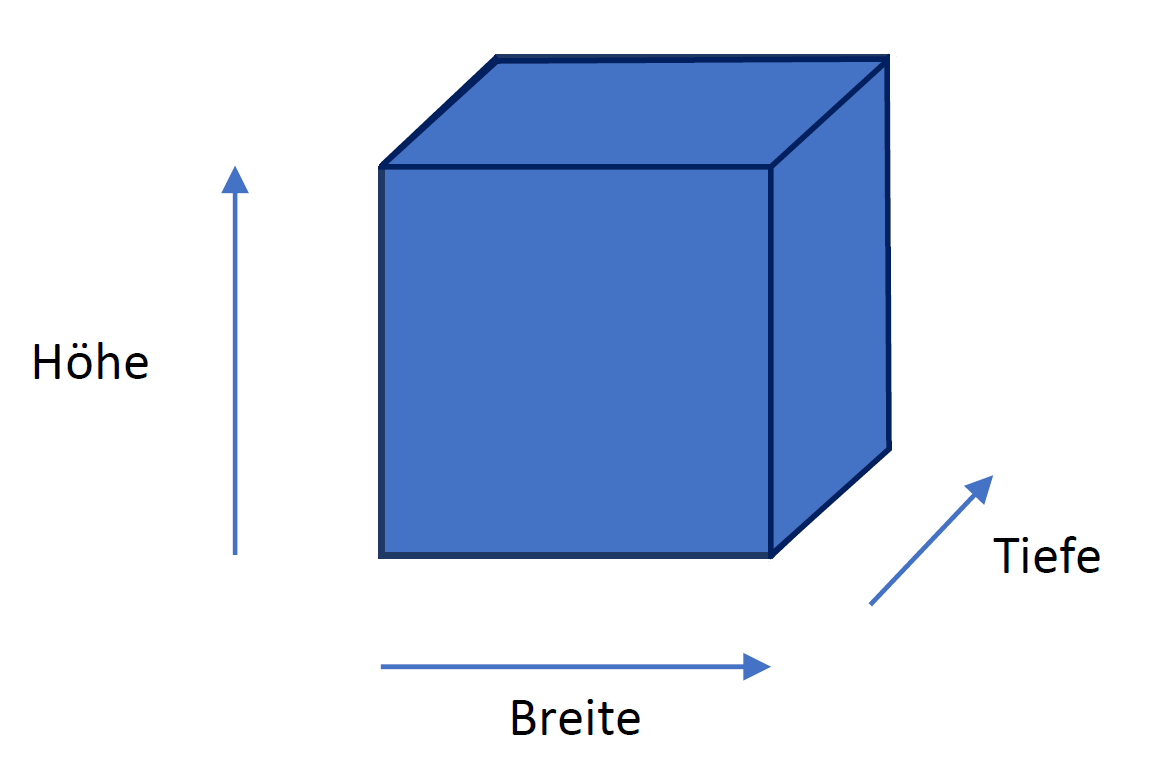
\includegraphics[scale=0.4]{pictures/grafiken/bht-erlk}
\label{fig:bth}
\caption{Visualisierung eines Tensors des 3. Ranges mit Zuordnung der Begrifflichkeiten.}
\end{figure}

\paragraph{Convolutional Layer}

Ein Convolutional Layer ist einer der Kernbestandteile eines CNNs. Der Layer verfügt über eine bestimmte Anzahl an Filtern, welche durch einen Tensor des selben Ranges wie die Eingabedaten bemessen werden. Filter sind durch ihre Reception Fields (zu Deutsch: rezeptive Felder) charakterisiert, welche die Größe der zeitgleich untersuchten Areale in den Eingabedaten bestimmen \parencite{DBLP:journals/corr/OSheaN15}. Ein Beispiel für das Reception Field eines Neurons könnte eine $M \times N$ große Fläche sein, welche kleinere oder gleich große Abmessungen haben sollte wie die Dimensionen der Eingabedaten. Das Reception Field spannt somit eine Matrix auf in der die Gewichte jedes Filters enthalten sind. In Abbildung \ref{fig:convbsp} spannt das Reception Field für einen Filter eine $2 \times 2$ Matrix, deren Gewichte alle 1 sind. Während der Filter die Eingabe verarbeitet, wird er über die Eingabematrix geschoben und multipliziert die Werte in dem untersuchten Bereich mit den Werten seines Filters. Die Produkte werden zu einem einzigen Werte aufsummiert, welcher dann den Wert für das Areal widerspiegelt. Wenn der Prozess endet, ist das Ergebnis eine etwas kleinere Matrix, in welcher die aufsummierten Ergebnisse für jede mögliche Position des Filters in den Eingabedaten erfasst sind. Sind in einem Layer mehrere Filter, so verfügt jeder Filter über eine individuelle Gewichtsmatrix mit gleichen Dimensionen. Jeder dieser Filter resultiert jeweils in einer Ausgabematrix. Bei zwei-dimensionalen $H \times W$ Eingabedaten -- mit $H$ = Höhe und $W$ = Breite -- werden die resultierenden Ausgabematrizen in der dritten Dimension $D$ (Tiefe) angeordnet, wobei $D$ = die Anzahl der verwendeten Filter ist. Die Ausgabe entspricht somit einem Tensor des Ranges 3.  

\begin{figure}[H]
\centering
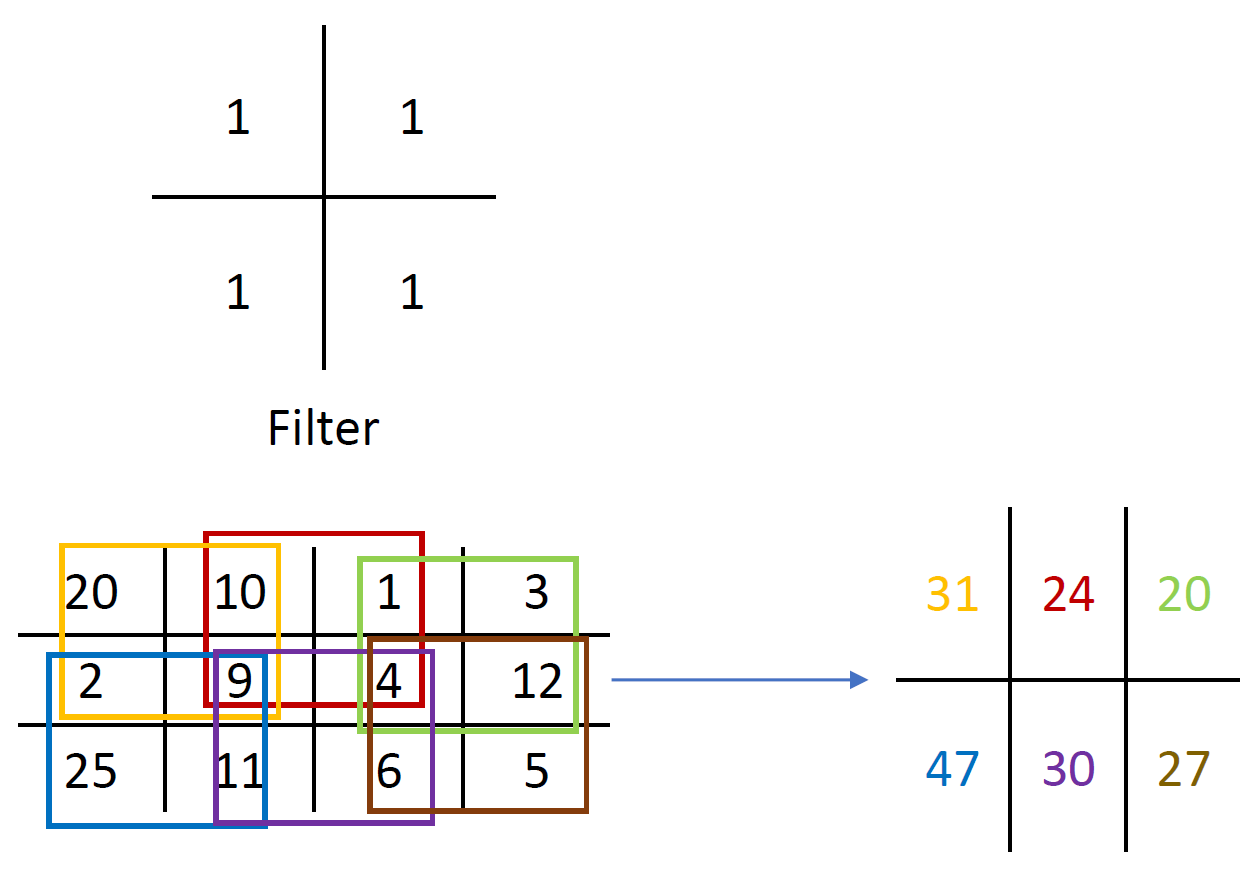
\includegraphics[scale=0.4]{pictures/grafiken/conv-bsp}
\label{fig:convbsp}
\caption{Ablauf einer Convolution mit einem $2 \times 2$ Filter und einer $3 \times 4$ großen Eingabematrix.}
\end{figure}

Nimmt man eine Matrix der Dimension $10 \times 10$ und führt auf dieser eine Convolution mit 5 Filtern und einem $5 \times 5$ Reception Field aus, so ist die Ausgabe des Convolution Layers ein Tensor des dritten Ranges mit Dimensionen $6 \times 6 \times 5$. 

Im Allgemeinen resultiert die Eingabe eines Tensors mit Bemessung $H^l \times W^l \times D^l$ und einem Filter der Größe $H \times W \times D^l \times D$ in einem Ausgabetensor der Dimension $(H^l - H + 1) \times (W^l - W + 1) \times D$. In dieser Notation verweist $l$ auf den vorherigen Layer \parencite{Wu.2017}.

Sollte eine Ausgabetensor mit den selben Dimensionen wie der Eingabetensor benötigt werden, so ist es möglich \textit{padding} (zu Deutsch in etwa: \textit{Polsterung}) zu nutzen, um der Matrix Spalten und Zeilen nach Bedarf hinzuzufügen. Um die Dimensionen des Eingabetensors zu erhalten, müssen $\lfloor \frac{H-1}{2} \rfloor$ Zeilen oberhalb der ersten Zeile und $\lfloor \frac{H}{2} \rfloor$ unterhalb der letzten Zeile hinzugefügt werden. Außerdem müssen $\lfloor \frac{W-1}{2} \rfloor$ Spalten vor der ersten Spalte und $\lfloor \frac{W}{2} \rfloor$ Spalten nach der letzten Spalte eingefügt werden. Der Notation der vorangegangenen Absätze folgend, beziehen sich $W$ und $H$ auf die vertikale und horizontale Dimension des Filters.

Zusätzlich kann ein \textit{stride}-Parameter (zu Deutsch: \textit{Schritt-Parameter}) $s$ definiert werden. Dieser Parameter bestimmt um wie viele Stellen der Filter nach jeder Rechnung auf dem Tensor verschoben wird. Wenn jede mögliche Position auf dem Tensor evaluiert werden soll, beträgt der Wert des stride-Parameters $s=1$. Für alle $s > 1$ wird der Filter $s - 1$ Positionen entlang beider Axen überspringen.

Der Vorgang des Abgehens der Eingabewerte kann durch eine mathematische Formel [\ref{eq:convolution}] beschrieben werden. In der Formel ist der stride-Parameter $s=1$ und es findet kein padding statt. $H^{l+1}$, $W^{l+1}$ und $D^{l+1}$ beziehen sich auf Höhe, Breite und Tiefe des Ausgabetensors.
 
\begin{equation}
y \in \mathbb{R}^{H^{l+1} \times W^{l+1} \times D^{l+1}}
\end{equation}

mit $H^{l+1} = H^l - H + 1$, $W^{l+1} = W^l - W + 1$, and $D^{l+1} = D$ \parencite{Wu.2017}.


\begin{equation}
\label{eq:convolution}
y_{i',j',di} = \sum_{i=0}^{H}\sum_{j=0}^{W}\sum_{d =0}^{D^l} f_{i,j,d,di} \cdot x^{l}_{i'+i, j'+j, d}
\end{equation}

$f$ ist ein Tensor des vierten Ranges mit den Indizes $ 0 \leq i < H,0 \leq j < W, 0 \leq d^l < D^l und 0 \leq d < D$ und stellt die Menge der Filter und deren Gewichte dar. $x^l$ ist die Ausgabe des vorherigen Layers. Die Gleichung \ref{eq:convolution} wird \"uber die komplette Tiefe $D^l$ der Eingabe wiederholt ($0 \leq di \leq D^l$). Sie wird lediglich auf Positionen $(i',j')$ angewandt, welche die Bedingungen $0 \leq i' < H^{l + 1}$ und $0 \leq j' < W^{l + 1}$ erfüllen \parencite{Wu.2017}.

\paragraph{Pooling layers}

Pooling Layer (zu Deutsch etwa: \textit{bündelnde Schicht}) werden auch als Downsampling Layer bezeichnet. Ihre Aufgabe besteht darin die Ausgabewerte des vorherigen Layers in einen Wert zu kombinieren und somit die Dimensionen der weitergereichten Daten zu reduzieren. Abbildung \ref{fig:maxpool} zeigt eine bildliche Erklärung des Maxpool Layers.

\begin{figure}[H]
\centering
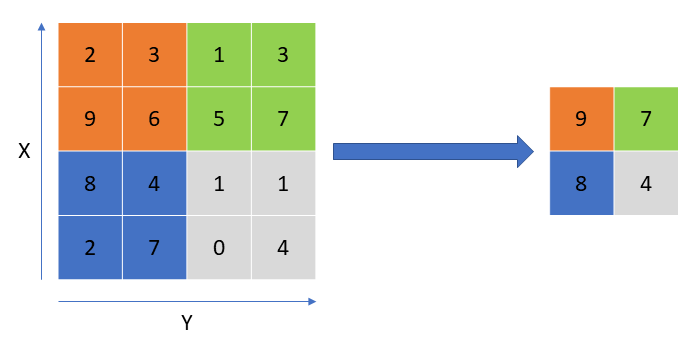
\includegraphics[scale=0.45]{pictures/grafiken/grafikenmax}
\caption[Caption for LOF]{Einfache Veranschaulichung des Maxpool Layers mit $2 \times 2$ stride-Parameter.}
\label{fig:maxpool}

\end{figure}

Der Maxpool Layer fußt auf der Idee, dass die exakte Position eines Merkmals nicht so wichtig ist, wie seine Position in Relation zu anderen Merkmalen. Abhängig von der gestellten Aufgabe könnte die Lage des Merkmals auch gar nicht relevant sein und die wichtige Information, die dieses Merkmal enthält ist lediglich seine Existenz. Ein Pooling Layer reduziert die Dimensionen des Eingabetensors in Abhängigkeit von seinen Parametern. So reduziert ein $2\times 2$ Pooling Layer eine $8\times8$ dimensionierte Eingabe auf die Dimension $4\times4$, da es die Eingabematrix in sich nicht überlappende $2\times2$ Quadrate unterteilt und f\"ur jedes Quadrat einen Wert errechnet, welcher in die Ausgabematrrix einflie\ss{}t. Die Inhalte der Ausgabe hängen von dem Typ des Layers ab, so errechnet ein Maxpooling Layer immer die größten Werte beobachteten Bereichs, ein Average Pooling Layer wiederum berechnet den Durchschnitt aller Werte in dem relevanten Bereich.

Der Pooling Layer arbeitet auf der kompletten Tiefe der Eingabe und reduziert diese daher nicht, sondern berechnet jede Matrix unabhängig von den anderen. Die Eingabe wird somit lediglich in Breite und Höhe reduziert. Obwohl es auch andere Varianten der Pooling Layer gibt, wie zum Beispiel Average Pooling oder L2-norm Pooling, wird hauptsächlich Maxpooling in den bekanntesten Architekturen verwendet.

Der Notation folgend resultiert ein Pooling Layer der Größe $(H \times W)$ in einer Ausgabe $H^{l+1} \times W^{l+1} \times D^{l+1}$. Unter der Annahme, dass $H$ und $W$, $H^l$ und $W^l$ teilen, gilt \parencite{Wu.2017}:

\begin{equation}
H^{l+1} = \frac{H^l}{H}, W^{l+1} = \frac{W^l}{W}, D^{l+1} = D^l.
\end{equation} 

Ein Maxpooling Layer kann wie folgt definiert werden:

\begin{equation}
y_{i', j', d} = \max_{0 \leq i<H, 0 \leq j <W} x^{l}_{i' \cdot H + i, j' \times W + j, d}
\end{equation}

es gilt $0 \leq i' < H^{l+1}, 0 \leq j' < W^{l+1}$, und $0 \leq d < D^{l+1} = D^l$.  